\documentclass[runningheads]{comsis2}

\usepackage[ruled,linesnumbered]{algorithm2e}
%\usepackage{algorithm}
%\usepackage{amssymb,amsthm,amsmath}
\usepackage{amssymb}
\usepackage{balance}
\usepackage{subfigure}
\usepackage{float}
%\newtheorem{theorem}{Theorem}[section]
%\newtheorem{lemma}[theorem]{Lemma}
\usepackage{latexsym}
\usepackage{multirow}
\usepackage{color}
\usepackage{url}
\usepackage{comment}
\usepackage[dvips]{graphicx}          % graphicx package for including ps files  

%% Necessary definitions for the running heads
\def\journalissue{Computer Science and Information Systems ?(?):??--??}
\def\paperidnum{DOI: N/A}
\setcounter{page}{1}

\title{MLPPI Wizard: An Automated Multi-level Partitioning Tool on Analytical Workloads}
%\titlenote{An earlier version of this article was presented as a short paper at ACM CIKM'12.}
%% Use this if the title is too long for the running heads
%\titlerunning{An Automated Multi-level Partitioning Tool on Analytical Workloads}

\author{Young-Kyoon Suh\inst{1} \and Alain Crolotte\inst{2} \and Pekka Kostamaa\inst{2}}
%Correspondence to Young-Kyoon Suh, now at Korea Institute of Science and Technology Information
%% Use this the list of authors is too long for the running heads
%\authorrunning{Correspondence to Young-Kyoon Suh, now at Korea Institute of Science and Technology Information}

\institute{Department of Computer Science, The University of Arizona, AZ 85721, USA\footnote{Currently, he is at Korea Institute of Science and Technology Information (KISTI). This work was conducted while he interned at Teradata during his PhD in the University of Arizona.}\\ 
  %\email{yksuh@cs.arizona.edu}
  \email{yksuh@cs.arizona.edu}
  \and
  Teradata Corporation, El Segundo, CA 90245, USA\\
  \email{\{alain.crolotte,pekka.kostamaa\}@teradata.com}
}

\def\form#1{$\langle{#1}\rangle$}
\def\range#1{$[{#1}]$}
\def\openrange#1{$({#1})$}
\def\lopenrange#1{$({#1}]$}
\def\ropenrange#1{$[{#1})$}
\def\product#1{$(#1)$}
\definecolor{grey}{RGB}{200,200,200}
\newcommand{\hilite}[1]{\colorbox{grey}{#1}}
\newcommand{\hilitey}[1]{\colorbox{yellow}{#1}}
\newcommand{\hiliting}[1]{\colorbox{grey}{#1}}
\long\def\todo#1{\hilitey{{\bf TODO:} {\em #1}}}
\long\def\shorten#1{}
\long\def\comment#1{}
\def\MAX{\mbox{\sl MAX}}
\def\LIMIT{\mbox{\sl LIMIT}}
\def\getQueryCost{\mbox{\sl getQueryCost}}
\def\getScanCost{\mbox{\sl getScanCost}}
\def\BigO{\mbox{\sl O}}
\def\NULL{\mbox{\sl NULL}}
\def\SolA{\mbox{\sl A}}
\def\SolB{\mbox{\sl B}}
\def\SolC{\mbox{\sl C}}
\def\SolS{\mbox{\sl S}}
\def\Qone{\mbox{\sl q1}}
\def\Qtwo{\mbox{\sl q2}}
\def\Sone{\mbox{\sl s1}}
\def\Stwo{\mbox{\sl s2}}
\def\SolSone{\mbox{\sl S1}}
\def\SolStwo{\mbox{\sl S2}}
\def\SolSthree{\mbox{\sl S3}}
\def\SolSfour{\mbox{\sl S4}}
\def\SolSfive{\mbox{\sl S5}}

\begin{document}

\maketitle

\begin{abstract} 
Typically, it is a daunting task for a database administrator (DBA) to figure out how to partition a huge fact table accessed by query workloads for better performance. To relieve such a burden, we introduce an intelligent partitioning tool to recommend an optimized partitioning on the fact table. This tool uses a greedy algorithm for search space enumeration. This space is driven by predicates of a given query workload. The tool takes advantage of the cost model of a query optimizer to prune the search space. The tool resides completely on a client and interacts with the optimizer via APIs. Thus, there is no overhead to instrument the optimizer code. Furthermore, the predicate-driven method can be applied to any clustering or partitioning scheme. We show that the tool's recommendation outperforms a human expert's solution. We also demonstrate that the recommendation scale very well with increasing workload and growing fact table.

\vspace{6pt}\textbf{Keywords:} Star Schema, Fact Table, Multi-Level Partitioning.
\end{abstract}

\section{Introduction}
\label{sec:intro}

Over the past decades much attention has been paid 
to improve the performance on analytical workloads in a data warehousing environment. 
Typically, a relational database management system (\hbox{DBMS}) 
has been exploited to process such analytical queries faster 
and assist its customers to make a timely business-decision in 
rapidly changing enterprise data warehousing.
Teradata DBMS has been a leading database product in this data warehousing marketplace 
that has been increasingly more competitive than ever.

%\subsection{Background}
%\label{sec:background}

\paragraph{Background:} 
To optimize the performance of analytical processing, 
tables and materialized views in the Teradata DBMS are hash-distributed based 
on a user-specified column or set of columns called {\em primary index}. 
Each virtual processor, a unit of parallelism called {\em AMP} in 
the \hbox{Teradata} \hbox{DBMS}, 
receives a subset of the data and stores it in hash order. 
Users typically choose primary index fields in the DBMS, 
so that the data is evenly distributed among the AMPs. 
The primary index fields are also chosen to reflect join fields 
in workloads to accomplish cheaper local joins that do not require data shuffling. 

Partitioned Primary Index (PPI)~\cite{sinclair:ppi} is an optional horizontal 
partitioning scheme applied locally on the data belonging to each AMP. 
In some database products, this type of partitioning is termed {\em clustering}, 
but hereafter we call the term \hbox{{\em partitioning}} only to avoid confusion.
Database \hbox{administrators} (DBAs) usually choose the columns for PPI, 
based on join fields and single table \hbox{predicates} to optimize the queries included 
in the workload. 
The PPI columns are used to physically group data with the same values 
together in contiguous data blocks. 
This grouping enables ``partition elimination'' in scans and joins for performance enhancement.
PPI can be specified as single or multiple levels. 
This type of partitioning scheme is known as 
\hbox{Multi-Level} PPI ({\em MLPPI)}~\cite{klindt09mlppi}.

By allowing non-qualified partitions to be eliminated, MLPPI can considerably 
reduce the amount of data to be scanned to answer a query. 
But a large number of partitions can create significant overhead, 
particularly in joins and table maintenance operations 
such as inserts and deletes, so that the selection of partitions can be usually a balancing act. 

Figure~\ref{fig:exam} exemplifies an MLPPI table with a defined partitioning option. 
This example is a subset of the {\tt LINEORDER} table from the Star Schema Benchmark (SSB)~\cite{oneil:ssb}. 
(Note that the full table with modified data types was actually used in our experiments.)

\begin{figure}[t]
\begin{center}
{\small
\begin{tabular}{l}
{\tt CREATE TABLE LINEORDER(} \\
\hspace{0.1in}{\tt LO\_ORDERKEY INTEGER,} \\
\hspace{0.1in}{\tt LO\_QUANTITY INTEGER,} \\
\hspace{0.1in}{\tt LO\_DISCOUNT INTEGER} \\
{\tt )} \\
{\tt PRIMARY INDEX ( LO\_ORDERKEY )} \\
{\tt PARTITION BY (} \\
\hspace{0.1in}{\tt CASE\_N(} \\
\hspace{0.2in}{\tt LO\_DISCOUNT >= 7,} \\
\hspace{0.2in}{\tt NO CASE OR UNKNOWN),} \\
\hspace{0.1in}{\tt CASE\_N(}\\
\hspace{0.2in}{\tt LO\_QUANTITY < 25,} \\
\hspace{0.2in}{\tt LO\_QUANTITY >= 25 AND LO\_QUANTITY <= 30,} \\
\hspace{0.2in}{\tt LO\_QUANTITY > 30 AND LO\_QUANTITY <= 35,} \\
\hspace{0.2in}{\tt NO CASE OR UNKNOWN)} \\
{\tt );} \\
\end{tabular}
}
\end{center}
\vspace{-0.2in}
\caption{An Example of an MLPPI Table in the Teradata DBMS\label{fig:exam}}
\end{figure}

In the definition of {\tt LINEORDER} in the figure, the primary index 
is on {\tt LO\_ORDERKEY}. 
The \hbox{primary} index \hbox{dictates} the AMP on which a row will be located 
while the partitioning of data will be dictated by the values and 
ranges associated with {\tt LO\_DISCOUNT} and {\tt LO\_QUANTITY}. 
For example, {\tt LO\_DISCOUNT} has two ranges: (i)~one for \hbox{values} $\geq$ 7 
and (ii)~another for all the other values (or {\tt NO CASE OR UNKNOWN}). 
{\tt LO\_QUANTITY} has four ranges. 
Hence, the relation will have a total of 2$\times$4 = 8 partitions as follows.

\begin{center}
{\footnotesize
\begin{tabular}{|c|l|}\hline 
Partition Number & Condition \\ \hline
1		& {{\tt LO\_DISCOUNT >= 7 \&\& LO\_QUANTITY < 25}} \\ \hline
2		& {{\tt LO\_DISCOUNT >= 7 \&\& 25 <= LO\_QUANTITY <= 30}} \\ \hline
3		& {{\tt LO\_DISCOUNT >= 7 \&\& 30 < LO\_QUANTITY <= 35}} \\ \hline
4		& {{\tt LO\_DISCOUNT >= 7 \&\& LO\_QUANTITY no case}}\\ \hline
5       & {{\tt LO\_DISCOUNT no case \&\& LO\_QUANTITY < 25}} \\ \hline 
6		& {{\tt LO\_DISCOUNT no case \&\& 25 <= LO\_QUANTITY < 30}} \\\hline								  	        
7		& {{\tt LO\_DISCOUNT no case \&\& 30 < LO\_QUANTITY <= 35}} \\ \hline
8		& {{\tt LO\_DISCOUNT no case \&\& LO\_QUANTITY no case}} \\ \hline
\end{tabular}
}
\end{center}

Whatever partition is chosen, 
the selection must be semantically correct; namely, 
the mapping of rows to partitions must be an injection. 
In other words, the constraints must form a covering of 
the entire range, so that a row will belong to exactly one and one partition. 
The Teradata optimizer then applies \hbox{partition} elimination for queries 
that specify conditions on {\tt LO\_DISCOUNT} and/or {\tt LO\_QUANTITY}. 
For \hbox{example}, only partitions~1 and~2 are needed for the query 
``{\tt SELECT * FROM LINEORDER WHERE} \linebreak {\tt LO\_DISCOUNT >= 7 AND} {\tt LO\_QUANTITY <= 30}.'' 
Similarly, partitions~1 and~5 are sufficient to answer the query 
``{\tt SELECT * FROM LINEORDER WHERE} \linebreak {\tt LO\_QUANTITY < 25}.'' 
The respective sizes of the partitions are a factor of the data distribution. 
To see MLPPI in greater detail, check our references~\cite{klindt09mlppi,sinclair:ppi}. 

%\vspace{-.1in}

%Next, using {\tt LINEORDER} defined in the SSB we provide examples of partitioning options that 
%a DBA may define based on a small query set. 
\paragraph{Challenge:}
Consider the below query set $Q$ having two queries $q$1 and $q$2 on the SSB.
\vspace{-.05in}
\begin{center}
{\small
\begin{tabular}{rl}
$q$1:	& {\tt SELECT SUM(l.LO$\_$EXTENDEDPRICE*l.LO\_DISCOUNT)} \\ 
		& {\tt FROM LINEORDER l, DDATE d} \\
		& {\tt WHERE l.LO\_ORDERDATE = d.D\_DATEKEY} \\
		& {\tt AND d.D\_YEAR = `1993'} \\
		& {\tt AND l.LO\_DISCOUNT IN (1, 4, 5)} \\
        & {\tt AND l.LO\_QUANTITY <= 30} \\ 
$q$2:	& {\tt SELECT c.C\_NATION, SUM(l.LO\_REVENUE)} \\ 
		& {\tt FROM CUSTOMER c, LINEORDER l} \\
		& {\tt WHERE l.LO\_CUSTKEY = c.LO\_CUSTKEY} \\
		& {\tt AND c.C\_REGION=`EUROPE'} \\
		& {\tt AND l.LO\_DISCOUNT >= 7} \\
		& {\tt AND l.LO\_QUANTITY >= 25 AND l.LO\_QUANTITY <= 35} \\
		& {\tt GROUP BY c.C\_NATION} \\
		& {\tt ORDER BY revenue desc} \\
\end{tabular}
}
\vspace{-.01in}
\end{center}

A DBA may focus on the {\tt LINEORDER} fact table and 
the predicates involving \linebreak {\tt LINEORDER} fields only. 
He can figure out the following five constraints, identified by the query number 
and the sequence number of predicates in each query: 
\vspace{-.05in}
\begin{center}
\begin{tabular}{cl}
$q$1.1: & {\tt LO\_DISCOUNT IN (1,4,5)} \\ 
$q$1.2: & {\tt LO\_QUANTITY <= 30} \\ 
$q$2.1: & {\tt LO\_DISCOUNT >= 7} \\ 
$q$2.2: & {\tt LO\_QUANTITY >= 25}\\ 
$q$2.3: & {\tt LO\_QUANTITY <= 35}. \\ 
\end{tabular}
\end{center}
\vspace{-.05in}
At this point the DBA needs to take into account options 
based only on two fields and the five constraints. 
There are many other possibilities from a {\em fine-grained} partition set 
to a {\em coarser-grained} definition. 

Considering for the time being the column {\tt LO\_DISCOUNT}, 
one solution is to identify each value 
for the {\tt IN} predicate in $q$1.1 
and use $q$2.1 as is. This yields the following partitioning expression 
for {\tt LO\_DISCOUNT}:
\vspace{-.05in}
\begin{center}
{\footnotesize
\begin{tabular}{l}
{\tt CASE\_N(} \\
\hspace{0.1in}{\tt LO\_DISCOUNT = 1,} \\
\hspace{0.1in}{\tt LO\_DISCOUNT = 4,} \\
\hspace{0.1in}{\tt LO\_DISCOUNT = 5,} \\
\hspace{0.1in}{\tt LO\_DISCOUNT >= 7,} \\
\hspace{0.1in}{\tt NO CASE OR UNKNOWN} \\
{)}. \\
\end{tabular}
}
\end{center}
This expression minimizes the size of the partitions 
by focusing exactly on the values required to satisfy the constraints 
but creates a large number of small partitions. 

Another possibility is to look at the maximum and minimum 
values in the {\tt IN} set and to build an {\tt AND} clause equivalent to 
a between clause yielding the following:
\vspace{-.1in}
\begin{center}
\begin{tabular}{l}
{\tt CASE\_N(} \\
\hspace{0.1in}{\tt LO\_DISCOUNT >= 1 AND LO\_DISCOUNT <= 5,} \\
\hspace{0.1in}{\tt LO\_DISCOUNT >= 7,} \\
\hspace{0.1in}{\tt NO CASE OR UNKNOWN} \\
{)}. \\
\end{tabular}
\vspace{-.1in}
\end{center}

\noindent The above partitioning solution decreases the number of partitions, 
compared to the previous solution but still focuses sharply on the constraints 
with still relatively small partitions. 

%(Another possibility would be to use the partitioning associated with {\tt LO\_DISCOUNT} shown 
%in the beginning of this section with only two partitions.)

Similar considerations apply to the partitioning associated with {\tt LO\_QUANTITY}. 
The resulting partitioning definition for the table includes both {\tt LO\_DISCOUNT}
and \linebreak {\tt LO\_QUANTITY}, and thus the number of possible combinations is the product of 
the potential combinations for each field. 

Furthermore, given two queries one partitioning scheme may be favorable for one query but not for the other, or vice versa. 
As a result, the DBA becomes faced with a daunting combinatorial search problem 
and no clear basis to decide on which combination is the best. 
This state of affairs begs for a {\em tool} for the DBA.

\paragraph{Solution:} 
To ease a burden of partitioning decision, 
we introduce a novel physical database design tool, called {\em MLPPI wizard}, 
designed to recommend an effective partitioning solution for a given workload.
%Indeed, the \hbox{wizard} is the first physical database design tool 
%developed at Teradata.
This tool uses a greedy algorithm for search space enumeration 
and is based on a general framework allowing general expressions, 
ranges and case expressions for partition definitions. 
%is particularly well-suited for an MLPPI definition. 
We emphasize that the \hbox{predicate-driven} algorithm used by the tool can be applied 
to {\em any} clustering or partitioning scheme based on simple fields and expressions or complex SQL predicates 
in an {\em arbitrary} DBMS. 
The wizard also borrows the optimizer's cost model 
to prune the search space and reach a final solution. 

\begin{figure*}[htp!]
\centering
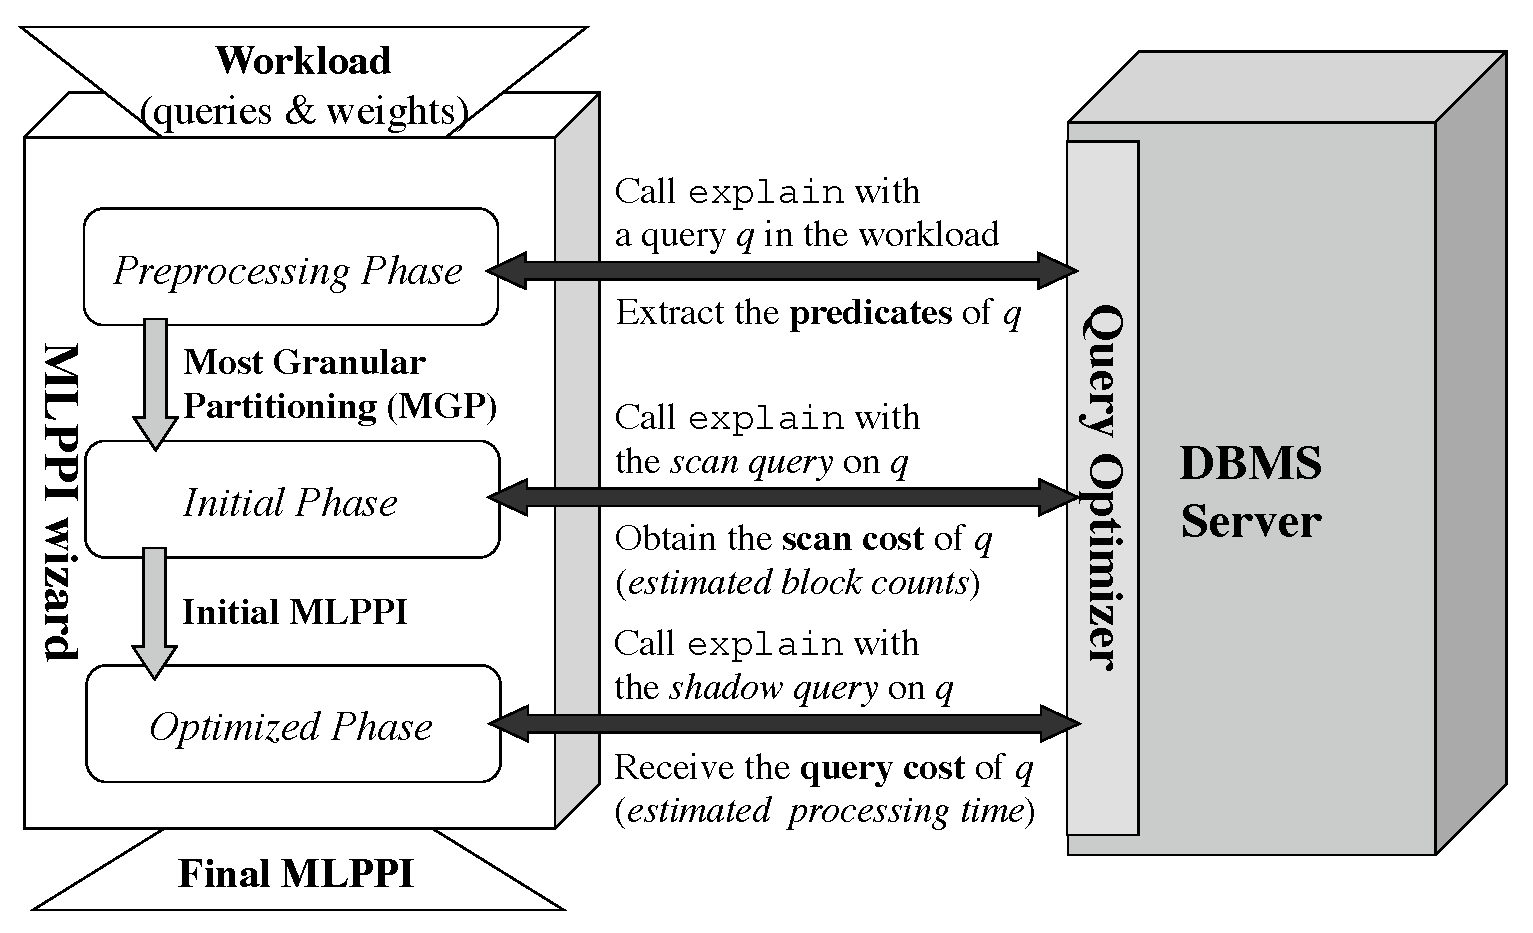
\includegraphics[scale=0.45]{architecture}
\vspace{-0.1in}
\caption{The MLPPI wizard architecture\label{fig:arch}}
\end{figure*}

Figure~\ref{fig:arch} illustrates how our tool recommends 
the final MLPPI customized for a given workload consisting of 
a set of queries and corresponding weights. 
Until yielding a final partitioning recommendation, 
the wizard passes through a series of phases: {\em Preprocessing}, 
{\em Initial}, and {\em Optimized} Phases. 
%In the pre-processing phase the tool produces the most granular partitioning (MGP) based on the predicates collected from every query.
%In the initial phase the wizard refines the passed MGP 
%by merging a pair of partitions with the least (scan) cost 
%and then yields an initial (feasible) MLPPI based on the refined partitions.
%In the \hbox{optimization} phase, the tool makes a further attempt to optimize the initial MLPPI. 
We elaborate in greater detail on each of the three phases, 
using the running query set $Q$ consisting of $q$1 and $q2$ in the rest of the article. 
As illustrated in Figure~\ref{fig:arch}, the wizard resides completely on the client side as opposed to 
several previous tools~\cite{agrawal04:integrating,Lightstone04:db2auto,nehme2011automated} 
that require optimizer code instrumentation. 
Our tool simply invokes the server's existing APIs used to simplify the queries, capture fact table 
predicates, and estimate processing costs. 
%This makes the wizard extensible and portable to different releases 
%of the Teradata DBMS server. 
%This \hbox{loosely-coupled} interaction 
%between both sides makes the wizard extensible and portable to different releases 
%of the database server. 
To the best of our knowledge, our wizard  
is the very first physical database design tool 
to address such a {\em \hbox{multi-level} partitioning} problem. 

\paragraph{Contribution:} This article provides 
the following contributions. 

\begin{itemize}
\item We propose a physical database design tool, termed MLPPI wizard, to recommend a multi-level partitioning definition 
for reducing the processing cost of a given query workload on a star schema benchmark. 
\item This tool is totally outside the database server, thereby incurring no overhead of instrumenting query optimizer's code.
\item We empirically show that a partitioning recommendation of our tool outperforms that of human expert 
over increasing workload size and growing fact table.

\end{itemize}

The article is a substantial extension of prior work~\cite{Suh12}. 
The rest of this article is \hbox{organized} in the following way. 
In the following section we propose a \hbox{multi-level} partitioning algorithm---consisting of a series of phases---used by our MLPPI wizard, 
which is applicable to any clustering or partitioning scheme in an arbitrary DBMS. 
In turn, we conduct a detailed analysis of the complexity of the algorithms. 
Next, we report the performance evaluation results. 
We then elaborate on how our wizard is distinguished from several existing tools proposed by other DBMS vendors. 
Finally, we conclude this article by summarizing our discussion.

\section{The MLPPI wizard}
\label{sec:algorithms}

As illustrated in Figure~\ref{fig:arch}, 
the MLPPI wizard has the three phases for a final partitioning recommendation. 
In this section we delve into each phase. For better exposition we use the running 
query set $Q$ \hbox{provided} in Section~\ref{sec:intro}.

\subsection{The Preprocessing Phase}
\label{sec:pre_phase}

The first phase is called {\em Preprocessing} 
to extract query predicates and check any constraint in partitioning. 
This phase consists of a total of six steps, as shown in Algorithm~\ref{algo:pre_phase}. 
%We elaborate on each step in the subsequent section.

%\vspace{-.1in}

\begin{algorithm}	
\caption{The Preprocessing Phase}
\label{algo:pre_phase}
\SetKwInOut{Input}{input}
\SetKwInOut{Output}{output}
\SetKw{func}{Function}
\SetKwBlock{begin}{}{end}
{
\Input{$Q$ (input query set) }
\Output{$R$ (non-overlapping range set), $M$ (query-to-range-set map)}
\hspace{.05in} Query Simplification (on $Q$)\\
\hspace{.05in} Range Extraction (from $Q$) \\
\hspace{.05in} Non-Overlapping Range ($R$) Construction \\
\hspace{.05in} Field Count Limit Check (on $R$) \\
\hspace{.05in} Query-to-Range-Set Map ($M$) Construction \\
\hspace{.05in} Partition Count Limit Check (on $R$) \\
}
\end{algorithm}

\subsubsection{Query Simplification}

The first step is to simplify the predicates of queries in a given workload.
In other words, we remove redundant conditions among the queries. 
For instance, if a query predicate has the condition of 
``{\tt LO\_DISCOUNT IN (1, 4, 5) AND LO\_DISCOUNT IN (2, 3, 4, 5)}'', 
then the predicate can be simplified as \linebreak ``\hbox{{\tt LO\_DISCOUNT}} {\tt IN (4, 5)}.'' 
This can be done via an API call to the database server. 
This simplification is not required for the running example.

%\vspace{-.3in}

\subsubsection{Range Extraction}

In the subsequent step we gather the simplified predicates and 
then extract ranges from the collected predicates. 
This task can also be performed through an API call to the server. 
The query predicate is of the form 
\begin{center}
\begin{tabular}{l} 
\form{\tt variable} \form{\tt op} \form{\tt constant},
\end{tabular}
\end{center}
where \form{\tt variable} is a field (column) from {\tt LINEORDER}, 
\form{\tt op} is in 
\begin{center}
\begin{tabular}{l} 
\{{\tt $ = $ }, {\tt $ < $}, {\tt $ <= $}, {\tt $ >= $}, {\tt $ > $}, 
{\tt IN}\},
\end{tabular}
\end{center}
and \form{\tt constant} represents a constant value(s). 
All \form{\tt op}s are self-explanatory. 
In particular, `{\tt IN}' is a list predicate implying `{\tt OR}' operator.
In the running example, 
we can collect a set of predicates $P$ = \{$p$1,$p$2,$p$3,$p$4\} from $Q$, where 

%\vspace{-.15in}

\begin{center}
\begin{tabular}{l} 
$p$1: {\tt l.LO\_DISCOUNT IN (1, 4, 5)} \\ 
$p$2: {\tt l.LO\_DISCOUNT >= 7} \\ 
$p$3: {\tt l.LO\_QUANTITY <= 30} \\ 
$p$4: {\tt l.LO\_QUANTITY >= 25} {\tt AND} {\tt l.LO\_QUANTITY <= 35}. \\ 
\end{tabular}
\end{center}

%\vspace{-.15in}

Next, we construct a bi-directional {\em map} between a query and 
associated predicates, so that for each query the corresponding predicate(s) 
can be found directly in the map, and vice versa. 
In the example, we get a map, called $M$1, built between $Q$ and $P$. 
$M$1 gets filled with the following entries:

$M$1:
\begin{center}
\begin{tabular}{ll} 
\form{q1, \{p1, p3\}} \\
\form{q2, \{p2, p4\}}.
\end{tabular}
\end{center}

Now we build a set of distinct ranges for each field referenced by the predicates. 
Specifically, we gather fields referenced by predicates in $P$, extract 
ranges from the predicates, and group the ranges of each of the referenced fields. 
Suppose $I$ to be a list of fact table fields referenced by $P$. 
In the workload $Q$ we add to $I$ two fields, {\tt LO\_DISCOUNT} and {\tt LO\_QUANTITY}, used by $P$. 
The whole range of the gathered predicates can be represented by a kind of two-dimensional array, called $R$. 

Each entry under a field in $R$ represents a pair of (start and end) values forming the range. 
When it comes to range representation for an entry, 
``['' and ``]'' are used for closed ranges while ``('' and ``)'' for open ranges. 
Also, infinity ($\infty$) and -infinity (-$\infty$) can be used for unbounded ranges. 
In particular, {\tt IN} predicate is represented by multiple ranges. 
For instance, the above $p$1 can be represented by the following three ranges 
\range{1, 1}, \range{4, 4}, \range{5, 5}; however, the last two consecutive 
ranges can be consolidated as \range{4, 5}. 
In the continuing example the field-wise distinct range set ($R$) is formed by the entries below.

$R$:
\begin{center}
\begin{tabular}{c|c} 
 {\tt LO\_DISCOUNT} & {\tt LO\_QUANTITY} \\ \hline
\range{1, 1} & \lopenrange{\infty, 30}\\
\range{4, 5} & \range{25, 35} \\
\ropenrange{7, \infty} &  \\
\end{tabular}
\end{center}

In turn, we build another map, called $M$2, between $P$ and $R$. 
That is, we associate each predicate in $P$ with a corresponding range in $R$. 
Let $R$[$i$, $j$] denote the interval value for the $i$-th field and $j$-th range in $R$. 
$R$[1, 3], for instance, indicates range \ropenrange{7, \infty} under {\tt LO\_DISCOUNT}. 
In the running example, $M$2 is constructed as follows:

$M$2:
\begin{center}
\begin{tabular}{l}
$\langle${$p$1}, \{$R$[1, 1],$R$[1, 2]\}$\rangle$ \\
$\langle${$p$2}, \{$R$[1 ,3]\}$\rangle$ \\ 
$\langle${$p$3}, \{$R$[2, 1]\}$\rangle$ \\
$\langle${$p$4}, \{$R$[2, 2]\}$\rangle$. \\
\end{tabular}
\end{center} 

\subsubsection{Non-Overlapping Range Construction}

Since there may be multiple predicates on the same field across queries, 
extracted ranges for the field may overlap each other. 
The overlapping ranges must be broken without any common portion, in order 
that we can consider a pair of consecutive, \hbox{non-overlapping} ranges for 
a merge in subsequent phases. 


\begin{algorithm}[t]
\caption{Splitting Overlapping Ranges}
\label{algo:split_overlap}
\SetKwInOut{Input}{input}
\SetKwInOut{Output}{output}
\SetKw{func}{Function}
\SetKwBlock{begin}{}{end}
{
\Input{$R$ having overlapping ranges}
\Output{$R$ with consecutive, non-overlapping ranges}
	\ForEach{field $i$ $\in$ $R$}{	
		$L$ $\leftarrow$ Get the range set of $i$ from $R$ and sort by start value \\
		$j$ = 0 \;
		\While{$j$ $<$ $|L|$-1}{
			$r_{j}$, $r_{j+1}$ $\leftarrow$ Adjacent ranges in $L$ \\
			\If{$r_{j}$.$end$ $\geq$ $r_{j+1}$.$start$}{
				Make a split by modifying values of $r_{j}$ and $r_{j+1}$. \\
				Insert into $L$ an intermediate range if any. \\
				Re-sort ranges in $L$ and reset $j$ to 0. \\
			}\lElse{$j$++;}
		}
		Update $R$ with the final $L$. 
	} 
}
\end{algorithm}

Algorithm~\ref{algo:split_overlap} describes the way of breaking 
the \hbox{overlap} of ranges. 
For each field, the algorithm 
gets associated ranges of each field and sorts them by start value. 
We then check whether or not adjacent ranges overlap each other.
If that is the case, we make a split between the ranges. 
In the example, the split is applied on the 
overlapping ranges, \lopenrange{\infty, 30} and \range{25, 35} in {\tt LO\_QUANTITY}. 
Subsequently, a common (or intermediate) range (\range{25, 30}) is created and inserted into the range set 
belonging to the {\tt LO\_QUANTITY} field, in order to fill the gap. 
$R$ is shown in the following.

{\it $R$}:
\begin{center}
\begin{tabular}{c|c} 
 {\tt LO\_DISCOUNT} & {\tt LO\_QUANTITY} \\ \hline
\range{1, 1}      & \openrange{\infty, 25} \\
\range{4, 5}      & \range{25, 30} \\
\ropenrange{7, \infty} & \range{31, 35} \\
\end{tabular}
\end{center}

The update of $R$ affects the existing map $M$2. 
In the running example, $p$3 and $p$4 influenced by the split get mapped to 
new range sets, \{$R$[2, 1], $R$[2, 2]\} and \{$R$[2, 2], $R$[2, 3]\}, respectively. 
Of course, the range sets corresponding to $p$1 and $p$2 referencing {\tt LO\_DISCOUNT} remain unchanged. 
As a result, in the running example we obtain the updated $M$2 in the following.

\pagebreak
$M$2:
\begin{center}
\begin{tabular}{l}
$\langle${$p$1}, \{$R$[1, 1],$R$[1, 2]\}$\rangle$ \\
$\langle${$p$2}, \{$R$[1, 3]\}$\rangle$ \\ 
$\langle${$p$3}, \{$R$[2, 1], $R$[2, 2]\}$\rangle$ \\
$\langle${$p$4}, \{$R$[2, 2], $R$[2, 3]\}$\rangle$. \\
\end{tabular}
\end{center} 

\subsubsection{Field Count Limit Check}

One question that occurs is what if a DBMS has 
a limit of fields that can be used for a partitioning definition. 
(In the case of Teradata DBMS, up to 64 fields can be allowed for 
an MLPPI definition.)
If the number of fields present in $R$ exceeds the field count limit, 
we determine which field(s) should be thrown away to satisfy the limit. 
(The star schema fact table we use has much fewer fields than the limit, 
and thus, this step will not be executed.)
To choose victim fields, our tool computes the weighted sum of 
{\em query cost}, to be discussed in Section~\ref{sec:opt_phase}, 
of queries regarding each field. 
The sum can be obtained by adding up every query cost on an MLPPI using 
only the ranges under the field. 
We incrementally discard a field with the largest sum of query cost 
until the limit is reached. 
Correspondingly, we can update the existing $M$2. 
One might say that such an MLPPI may not be exploited if too many ranges 
over a partition count limit (65,536 in Teradata DBMS) are found in one field.
But we assume that such an extreme case is not expected. Even if 
such a case happens, the merges of consecutive ranges can make the MLPPI feasible. 

\subsubsection{Query-to-Range-Set Map Construction}

Using the existing maps $M$1 and $M$2, 
the tool can create the final bi-directional {\em query-to-range-set} map, say $M$, 
between $Q$ and $R$. 
To construct $M$, we leverage a transitive property from $M$1 to $M$2.
Once we compute $M$, there is no need to keep 
the intermediate maps ($M$1 and $M$2) for the subsequent phases. 
In the running example, we can build $M$ in the following. 

\pagebreak

{\it $M$}:
\begin{center}
\begin{tabular}{ll} 
$\langle${$q$1}, \{$R$[1, 1], $R$[1, 2], $R$[2, 1], $R$[2, 2]\}$\rangle$ \\
$\langle${$q$2}, \{$R$[1, 3], $R$[2, 2], $R$[2, 3]\}$\rangle$.
\end{tabular}
\end{center} 
\vspace{-.1in}
\noindent In the subsequent phases $M$ gets used for computing costs and updated 
along with a merge of ranges, and $R$ is refined for an MLPPI recommendation. 

\subsubsection{Partition Count Limit Check}

The range set $R$ can be used to define an MLPPI using each field as one level. 
However, if the current number of partitions by $R$ is greater than 
the aforementioned partition count limit, 
then it is not possible to make a feasible MLPPI based on the ranges in $R$. 

The actual partition count limit is ample enough to pass the running example, 
but to continue our discussion, assume that in our discussion the limit is {\it 15}.
From $R$ in the running example, we obtain a total of (number of ranges in {\tt LO\_DISCOUNT}) 
$\cdot$(number of ranges in {\tt LO\_QUANTITY}) = (3+1) $\cdot$ (3+1) = {\it 16}
partitions. Note here that one reserved range covering the rest but the identified 
is added by default to each field in the calculation, 
and the default range is equivalent to the ``{\tt NO CASE OR UNKNOWN)}'' case in Figure~\ref{fig:exam}. 
Since the total partitions surpass the limit, 
the tool should go through the initial phase in which 
we make fewer partitions than the limit. 
(Otherwise, the wizard can bypass the initial phase and then immediately proceed to the optimized phase.) 

The tool is now ready to proceed to the next phases, 
with $R$ (input range set, or MGP) and the prepared $M$ (query-to-range-set map). 
%In the following subsections, we describe how the MLPPI solution for $Q$ 
%can be eventually made using $M$ and $R$.

\subsection{The Initial Phase}
\label{sec:init_phase}

This phase incrementally merges a range pair in $R$ to reduce partitions. 
The merge continues until the number of ongoing partitions 
drops below the partition count limit. 
After finishing the merge, the tool can derive a feasible MLPPI with the remaining partitions. 

Overall, I/O cost may be increased by the merge, 
in that the full scan on a partition is performed to retrieve all the rows potentially matching a given query. 
In the case of a merged partition, we may read the non-qualifying rows 
that would not be seen before the merge, thereby paying more I/O to answer 
the query. To minimize the merge overhead, we pick up the range pair incurring 
the least I/O increase in a heuristic fashion. 
To choose a range pair for a merge, 
we calculate the {\em scan cost} of a query on the merged range pair.

Algorithm~\ref{algo:comp_scan_cost} represents how 
the scan cost can be computed on the range pair that \hbox{influences} a given query. 
The scan cost represents the I/O cost to answer the query when the range pair is merged. 
It is defined as the {\em number of blocks} that are to be read 
for the given query. To compute the scan cost of a query $q$, we write 
a corresponding scan cost query ($s$), which can be constructed as follows: 
\vspace{-.1in}
\begin{center}
$s$: {\tt SELECT * FROM $F$ WHERE} {\it CP},
\end{center} 
\vspace{-.1in}
where $F$ is a fact table, and 
{\it CP} indicates a predicate(s) reconstructed from 
a range(s) mapped to $q$ in $M$.

\begin{algorithm}[t]
\caption{Scan Cost Computation}
\label{algo:comp_scan_cost}
\SetKwInOut{Input}{input}
\SetKwInOut{Output}{output}
\SetKw{func}{Function}
\SetKwBlock{begin}{}{end}
{
\Input{$q$ (query), $rp$ (range pair), $M$ (query-to-range-set map)}
\Output{Scan cost for answering $q$ when considering a merge of $rp$}
	$r_{m}$ $\leftarrow$ Consolidate $rp$ \;
	$L$ $\leftarrow$ Copy the range set mapped to $q$ from $M$\; 
	Delete ranges in $rp$ from and insert $r_{m}$ into $L$. \\
	$s$ $\leftarrow$ ``{\tt SELECT * FROM FACT$\_$TABLE WHERE }'' \;
	\ForEach{range $r$ $\in$ $L$}{	
		Reconstruct a predicate $p$ from $r$. \\
		Add $p$ to {\tt WHERE} clause of $s$.
	}
	Make an API call with $s$ to the server. \\
	Extract the spool size (in bytes) from the result. \\
	$blc$ $\leftarrow$ Calculate the block counts from the spool size. \\
	Update $q$'s scan cost to $blc$. \\
	{\bf return} $blc$ \;
}
\end{algorithm}

If $q$ turns out being affected by the merge of a range pair, 
then the range set associated with $q$ in $M$ is temporarily updated 
by removing the parent ranges and adding the merged range. 
The altered range set is remapped to $q$ in $M$ and then 
translated to the equivalent predicates. Then {\it CP} for $s$ can be built based on the predicates.
Unless the merge range pair influences $q$, 
we can simply derive {\it CP} from the existing ranges mapped to $q$.

To see in the Algorithm~\ref{algo:comp_scan_cost} how a scan cost query is built, 
consider a range pair ($rp$) of \hbox{$R$[2, 2]} and $R$[2, 3] in the running example. 
$rp$ produces the merged range, \range{25, 35}, \hbox{under} {\tt LO\_QUANTITY}. 
The merge by $rp$ affects both $q$1 and $q$2 in the workload. 
Thus, the range sets of $q$1 and $q$2 on {\tt LO\_QUANTITY} are 
correspondingly altered to \{\openrange{\infty, 25}, \range{25, 35}\} and \{\range{25, 35}\}, 
respectively. Of course, no change is made to the existing range sets 
of the queries on {\tt LO\_DISCOUNT}. 
Therefore, the corresponding scan cost queries for $q$1 and $q$2 
can be built as shown below:
\vspace{-.05in}
\begin{center}
\begin{tabular}{rl}
$\Sone$:	& {\tt SELECT * FROM LINEORDER l} \\
		& {\tt WHERE ((l.LO\_DISCOUNT = 1) OR}\\
		& {\tt (l.LO\_DISCOUNT >= 4 AND l.LO\_DISCOUNT <= 5))} \\
		& {\tt AND l.LO\_QUANTITY <= 35}  \\ 
$\Stwo$:	& {\tt SELECT * FROM LINEORDER l} \\
        & {\tt WHERE l.LO\_DISCOUNT >= 7} \\
        & {\tt AND (l.LO\_QUANTITY >= 25 AND l.LO\_QUANTITY <= 35)}.
\end{tabular}
\end{center} 
\vspace{-.05in}
\noindent Since the altered ranges (\openrange{\infty, 25} and \range{25, 35}) of $q$1 
are consecutive, we can simply build the merged, single predicate ({\tt l.LO\_QUANTITY <= 35}) for $\Sone$. 

In turn, the wizard sends each scan cost query to the server through an API call. 
The tool extracts from the server's response the {\em spool size} (in bytes), which is 
the result size of the sent scan cost query, and then 
calculates as scan cost the {\em block counts} ($blc$) using the spool size. 
If the merge of a range pair does not impact on any query in the workload, 
the existing (previously computed) scan cost of queries is reused for the range pair. 
In other words, the wizard only recomputes the scan cost of a query {\em only if} 
the query is affected by the merge of two consecutive ranges. 
The weighted sum of scan cost of queries, $T_{s}$ can be computed 
for each range pair. 
$T_{s}$ can be defined as follows:
\begin{center}
\begin{tabular}{c} 
$T_{s}$ = $\sum_{i=1}^{n}$($sc_{i}${$\cdot$}{$w_{i}$}),
\end{tabular}
\end{center}
where $n$ is the number of queries in $Q$, $sc_{i}$ is the scan cost of a query $q_{i}$ in $Q$, and 
$w_{i}$ denotes the (\hbox{non-negative}) weight associated with $q_{i}$. 

Once all range pairs are examined, the tool chooses the range pair 
with the least $T_{s}$ for a merge. 
If several range pairs end up with the same least $T_{s}$, 
then the tool applies the heuristic of favoring the range pair that produces 
fewer number of partitions when merged, to make 
it faster to reach the partition count limit. 

In the example, suppose that the running range pair $rp$ produces the least $T_{s}$, 
and thus, the tool merges $rp$. 
Thus we can update both $R$ and $M$ as follows.

$R$:
\begin{center}
\begin{tabular}{c|c} 
{\tt LO\_DISCOUNT} & {\tt LO\_QUANTITY} \\ \hline
\range{1, 1} & \openrange{\infty, 25} \\
\range{4, 5} & \range{25, 35}		  \\
\ropenrange{7, \infty} &  \\
\end{tabular}
\end{center}

\vspace{-0.1in}
$M$:
\begin{center}
\begin{tabular}{ll} 
$\langle${$q$1}, \{$R$[1, 1], $R$[1, 2], $R$[2, 1], $R$[2, 2]\}$\rangle$ \\
$\langle${$q$2}, \{$R$[1, 3], $R$[2, 2]\}$\rangle$
\end{tabular}
\end{center} 

Note that we see that $q$2 may have the most customized partition based on the updated $M$. 
Only the single partition formed by ($R$[1, 3]$\cap${$R$[2, 2]}) is sufficient 
to retrieve all the qualifying 
rows for $q$2; thus, the other partitions can be simply eliminated. 
In the meantime, to answer $q$1, we need to read the four partitions formed by 
the top two ranges of each field. 
As the partitions formed by (({$R$[1, 1]{$\cup$}$R$[1, 2]})$\cap$($R$[2, 2]) 
contain the \hbox{non-qualifying} rows for $q$1, unfortunately, 
$R$ cannot provide $q$1 with as much benefit as $q$2. 
$R$, however, can be a good compromise to satisfy both queries, in that 
the MLPPI derived by $R$ can potentially minimize the total execution cost of $Q$. 

Algorithm~\ref{algo:init_phase} represents the initial phase 
that has been described so far. 
Given a \linebreak \hbox{query-to-range} set map ($M$) and an input range set ($R$), 
the algorithm determines which range pair to yield the least total execution cost ($T_{s}$) 
and updates $M$ and $R$ using the chosen range pair, 
until the number of the partitions by $R$ falls below a pre-defined partition limit count.
Finally, the algorithm produces the final recommendation based on $R$.

\begin{algorithm}[t]
\caption{The Initial Phase}
\label{algo:init_phase}
\SetKwInOut{Input}{input}
\SetKwInOut{Output}{output}
\SetKw{func}{Function}
\SetKwBlock{begin}{}{end}
{
\Input{$M$ (query-to-range-set map), $R$ (input range set)}
\Output{$R$ with \# partitions $\leq$ partition limit}
	$W$ $\leftarrow$ Query weights \\
	\While{(\# partitions by $R$ $>$ partition limit)}
	{
		\ForEach{a range pair ($rp$) in $R$}
		{	 
			$T_{s}$ $\leftarrow$ 0 \;
			\ForEach{$q$ in $M$}
			{	
				$w$ $\leftarrow$ Get $q$'s weight from $W$ \\
				$L$ $\leftarrow$ Get the range set mapped to $q$ in $M$ \\
				\uIf(\tcp*[f]{Affected}) {(($rp$ $\cap$ $L$) $\neq$ $\varnothing$)}
				{
					$T_{s}$ += $w{\cdot}$({\it getSC}($q$,$rp$,$M$)) \tcp*[r]{See Algo.~\ref{algo:comp_scan_cost} regarding {\it getSC}()}
				}
				%\lElse{ $T_{s}$ += $w{\cdot}$($q$'s existing scan cost)}
			}
			Associate $T_{s}$ with $rp$.
		}
		Find $rp$(s) with the least $T_{s}$. \\
		If a tie happens, select the $rp$ to make fewer partitions when consolidated. \\
		Update $M$ and $R$ by the chosen $rp$.
	}
	{\bf return} $R$\;
}
\end{algorithm}



In the running example the total partition counts ($4${$\times$}$3$=$12$) by $R$ is under 
the assumed limit ($15$), which meets the partitioning limit. 
Hence, the wizard can enter the optimized phase with $R$, 
without repeating the initial phase. 

\subsection{The Optimized Phase}
\label{sec:opt_phase}

%We verified the effectiveness of the tool by running it on a workload based
After passing the initial phase, 
we now have an initial MLPPI recommendation based on $R$, for the {\tt LINEORDER} fact table.
The initial recommendation can be used sufficiently. 

But we emphasize that additional merges may make fewer partitions, 
which actually can enhance the overall workload performance for the following reasons. 
First, multiple file contexts by many partitions can incur 
huge overhead that impacts on the query optimizer. 
There also exists an operational threshold 
that the optimizer can handle the maximum number of the partitions at a time.
Therefore, further reducing partitions greatly helps the optimizer to manage these partitions.

A similar algorithm, as suggested in the initial phase, 
can be applied. 
In this phase, we use {\em query cost}, analogous to scan cost, 
which can be obtained via a feasible MLPPI. 
Specifically, the query cost is modeled as the estimated processing time 
of a query on a {\it faked} fact table applying the MLPPI definition that reflects the merge of a range pair. 
This cost estimation technique is similar 
to the ``\hbox{what-if}" approach~\cite{chaudhuri1998autoadmin}.

\begin{algorithm}[t]
\caption{Query Cost Computation}
\label{algo:comp_query_cost}
\SetKwInOut{Input}{input}
\SetKwInOut{Output}{output}
\SetKw{func}{Function}
\SetKwBlock{begin}{}{end}
{
\Input{$q$ (query), $rp$ (range pair), $M$ (query-to-range-set map), $R$ (input range set)}
\Output{Query cost to answer $q$ when considering a merge of $rp$}
	Create an empty shadow table $H$ having the same definition as the fact table $F$, 
	including indexes and all constraints (check and referential integrity constraints). \\
	Propagate all (field and index) statistics of $F$ to $H$. \\
	\If{$F$ has materialized views (MVs)}{
		Create the equivalent MVs on $H$. \\
		Propagate the statistics of the MVs on $F$ to those of $H$. \\
	}
	$r_{m}$ $\leftarrow$ Merge $rp$ \;
	$L$ $\leftarrow$ Copy ranges associated with $q$ from $M$\; 
	Remove ranges in $rp$ from and add $r_{m}$ to $L$. \\
	$R'$ $\leftarrow$ Update $R$ with $L$ \\
	Alter $H$ using a fictitious MLPPI with $R'$. \\
	Construct and send to the server an $H$-based shadow query $h$ equivalent to $q$. \\	
	$ept$ $\leftarrow$ Estimated processing time of $h$ extracted from the server response \;
	Update $q$'s query cost to $ept$. \\
	{\bf return $ept$} 
}
\end{algorithm}

\begin{algorithm}[t]
\caption{The Optimized Phase}
\label{algo:opt_phase}
\SetKwInOut{Input}{input}
\SetKwInOut{Output}{output}
\SetKw{func}{Function}
\SetKwBlock{begin}{}{end}
{
\Input{$M$ (query-to-range-set map), $R$ (input range set)}
\Output{The MLPPI on which the total query cost is minimal}
	$W$ $\leftarrow$ Query weights \\
	$T_{p}$ $\leftarrow$ Total query cost sum on an initial MLPPI by $R$ \\
	\While{(Pre-defined iterations or $R$ $\neq$ $\varnothing$)}{
		\ForEach{range pair $rp$ in $R$}{	 
			$T_{q}$ $\leftarrow$ 0 \;
			\ForEach{$q$ in $M$}{	
				$w$ $\leftarrow$ Get $q$'s weight from $W$ \\
				$L$ $\leftarrow$ Get the range set mapped to $q$ in $M$ \\
				\uIf(\tcp*[f]{Affected}) 
				{(($rp$ $\cap$ $L$) $\neq$ $\varnothing$)}{
					$T_{q}$ += $w${$\cdot$}({\it getQC}($q$,$rp$,$M$,$R$)) 	
					\tcp*[r]{See Algo.~\ref{algo:comp_query_cost} regarding {\it getQC}()}				
				}
				\lElse{ $T_{q}$ += $w${$\cdot$}($q$'s existing query cost)}
			}
			Map $T_{q}$ to $rp$.
		}
		$T$ $\leftarrow$ The least $T_{q}$ that has been so far seen.  \\
		\lIf{$T$ $>$ $T_{p}$}{ {\bf break} \;}
		\Else{
			$T_{p}$ $\leftarrow$ $T$ \tcp*[r]{Query Cost Sum Update} 
			Find $rp$(s) with $T$. \\
			If a tie happens, select the $rp$ to make fewer partitions when consolidated. \\
			Update $M$ and $R$ by the chosen $rp$. \\
		}
	}
	{\bf return} an MLPPI by $R$ \;
}
\end{algorithm}

Algorithm~\ref{algo:comp_query_cost} illustrates the steps for computing the query cost of a query $q$. 
Given a range pair ($rp$) affecting $q$ when merged, 
we first create an empty shadow table $H$ with the same definition as $F$, 
including all indexes and constraints such as check and referential integrity 
ones. Next, we propagate all statistics of $F$ to $H$. 
This covers field and index statistics. 
If $F$ has materialized views (MVs), then we create the equivalent MVs on $H$ and subsequently, 
propagate the statistics of the MVs on $F$ to the new MVs on $H$. 
After that, we alter $H$ by an MLPPI with the updated $R$ ($R$'), applying the merge of $rp$. 
The algorithm then builds a {\em shadow} query $h$, equivalent to the input query $q$,
which is built by replacing $F$ in $q$ with $H$. 
The algorithm in turn makes an API call to the {\tt EXPLAIN} tool with $h$. 
Eventually, the algorithm extracts from the result and returns the estimated elapsed time 
of $h$ as the query cost of $q$. 
As done in the initial phase, the query cost of a query is recomputed only if the merge affects the query.

Algorithm~\ref{algo:opt_phase} proposes the algorithm of the optimized phase. 
$W$ indicates a set of weights assigned to individual queries in a given workload. 
$T_{p}$ keeps track of the existing least query cost sum, and initially is computed on an initial MLPPI. 
For each range pair, the algorithm 
computes the respective weighted sum ($T_{q}$) of query costs of the queries in a given workload. 
($T_{q}$ can be similarly defined as $T_{s}$, described in Section~\ref{sec:init_phase}, 
and thus the definition of $T_{q}$ is omitted here.)
Let the current least $T_{q}$ be $T$. 
If $T$ $<=$ $T_{p}$ (existing least), then for the next iteration $T_{p}$ is updated to $T$. 
We perform the merge on the range pair that produces that $T$ and update $M$ and $R$ along with the merge. 
The algorithm repeats the process until (1)~no more ranges in $R$ are left, or (2)~predefined iterations are reached. 
If $T$ $\geq$ $T_{p}$, then the optimized phase is terminated.

Note that to break a tie between range pairs, 
we apply the same heuristic to favor one of them that produces fewer partitions. 
The order of the different partitioning levels may have some impact on 
the execution time. A range condition on lower levels like the query 
in Section~\ref{sec:intro} 
``{\tt SELECT * FROM LINEORDER WHERE LO\_QUANTITY < 25}'' 
requires scanning non-consecutive partitions. 
This may incur some overhead at run time. 
To reduce this effect, we sort the partition levels based on the number of 
partitions in descending order before making the final recommendation. 
The solution in Figure~\ref{fig:exam} follows this heuristic 
making the two-partition case in the first level 
followed by the four-partition case in the second level. 
The order in Figure~\ref{fig:mlppi} can go \hbox{either} way 
since both levels have the same number of \hbox{partitions}.

In the running example, suppose that in the first round, ranges $R$[1, 1] and $R$[1, 2] are chosen for a merge. 
Then, the wizard produces a merged range \range{1, 5} \hbox{under} {\tt LO\_DISCOUNT} and proceeds to the next round. 
If a range pair selected for the subsequent merge fails to improve $T_{p}$, 
then, the tool exits the optimized phase and \hbox{produces} the final MLPPI recommendation for the given workload $Q$ 
as shown in Figure~\ref{fig:mlppi}. 

\vspace{-.25in}
\begin{figure}[h!]
\begin{center}
\begin{tabular}{|l|} \hline
{\tt ALTER TABLE LINEORDER} \\
{\tt MODIFY PRIMARY INDEX} \\
{\tt PARTITION BY(} \\
\hspace{.1in}{\tt CASE\_N(} \\
	\hspace{.2in}{\tt LO\_DISCOUNT $\geq$ 1 AND LO\_DISCOUNT $\leq$ 5,} \\
	\hspace{.2in}{\tt LO\_DISCOUNT $\geq$ 7,} \\ 
	\hspace{.2in}{\tt NO CASE OR UNKNOWN),} \\
\hspace{.1in}{\tt CASE\_N(} \\
	\hspace{.2in}{\tt LO\_QUANTITY $<$ 25,} \\
	\hspace{.2in}{\tt LO\_QUANTITY $\geq$ 25 AND LO\_QUANTITY $\leq$ 35,} \\
	\hspace{.2in}{\tt NO CASE OR UNKNOWN)} \\ 
{\tt );} \\ \hline
\end{tabular}
\end{center}
\vspace{-.2in}
\caption{The Final MLPPI Recommendation for the Given Workload $Q$\label{fig:mlppi}}
\vspace{-.2in}
\end{figure}

\section{Analysis}
\label{sec:analysis}

In this section we analyze the time complexity of 
the proposed algorithms: preprocessing, initial, and optimized phases. 
The metric of this complexity analysis on each phase is the logical running time of the wizard, 
equivalent to the number of API calls made to the database server during that phase. 

\subsection{The Preprocessing Phase}

\begin{lemma}
\label{lemma:pre_phase}  
The running time complexity for building a query-to-range map is 
$\BigO$($N${$\cdot$}$C${$\cdot$}$V$), where $N$ is the number of queries 
in a workload, $C$ is the total number of fields in the fact table, 
and $V$ is the max number of values in a field. 
\end{lemma}

{\bf Proof}. Consider the worst case such that given a workload of 
$N$ queries, each query references all the fields of the fact table, and 
each field is associated with at most $V$ values by the predicates of the queries. 
Each query may have a single-value range. 
A range consisting of only one value per field can be mapped to each query. 
Thus, the running time complexity for the map construction 
is $\BigO$($N${$\cdot$}$C${$\cdot$}$V$). \qed

But note that in our experiments the bound of $\BigO$($N${$\cdot$}$C${$\cdot$}$V$) 
was overly pessimistic. 

\subsection{The Initial and Optimized Phases}

\begin{lemma}
\label{lemma:init_phase}  
The running time complexity for the initial (or optimized) phase is 
$\BigO$($M^{2}${$\cdot$}$N$), 
where $M$ is the number of range pairs, and $N$ is the number of queries in a workload. 
\end{lemma}

{\bf Proof}. Suppose that the merge of every range pair influences all the queries. 
Every iteration, either the scan or query costs need to be recomputed for each query. 
In the first round we pay the \hbox{re-computation} cost of $M${$\cdot$}$N$ 
and merge a victim range pair. In the subsequent round, $M$-1 range pairs remain, 
so the cost amounts to ($M$-1){$\cdot$}$N$. 
In the worst case we end up consolidating all range pairs, thus having no partition on 
the target table. The total calls made to the server can be added up to 

\begin{center}
$M${$\cdot$}$N$+($M$-1){$\cdot$}$N$+$\cdots$+$N$ = ($\sum_{i=1}^M i$){$\cdot$}$N$ = $\frac{M(M-1)}{2}${$\cdot$}$N$. 
\end{center}

\noindent Hence, the running time complexity is $\BigO$($M^{2}${$\cdot$}$N$). $\qed$

%\vspace{0.1in}

Again, our experiments showed that $\BigO$($M^{2}${$\cdot$}$N$), the running time complexity, 
was overly pessimistic. Specifically, 
the number of calls made in our experiments was by far fewer than that bound. 
That was because it was very rare for a range pair to involve all queries in a given workload 
(as seen in Table~\ref{tab:workload_stat}).

%In the following we evaluate the performance of our wizard using the proposed algorithms.

\section{Experiment}
\label{sec:experiment}

In this section we evaluate the performance of our wizard using the proposed algorithms.
We first describe our environment settings. 
We then report the statistics measured during our experiments. 
Finally, we compare the performance of the recommendation 
by the MLPPI wizard (WIZARD) with (1)~that of no partitioning (NO PPI)
and (2)~the partitioning of a human expert (EXP) under different setups.

\subsection{Environment Settings}
\label{sec:env_set}

\paragraph{Development:} 
We implemented our MLPPI wizard as a prototype on top of the \hbox{Teradata} DBMS server. 
The wizard was written in Java. 
We evaluated the performance of the \hbox{wizard} 
on the Teradata DBMS server machine running Unix. 

\paragraph{Workload:} When it comes to workload generation, we took advantage of 
our simple star schema query \hbox{generator}. 
The generator assumes that (i)~available operators, (ii)~fields, 
and (iii)~the minimum and \hbox{maximum} values of the fields are already known. 
For each query, the generator first randomly selects the number of single-table 
predicates to create. 
The generator then arbitrarily chooses a field and a specific operator 
for each predicate. 
If {\tt IN} operator on a chosen field is picked up, the query generator 
determines the number of values to add to the {\tt IN} list and then chooses random values within the min-max value 
range of the field. 
In this way the generator makes a query involving the generated predicates.

A generated query is based on a template that joins {\tt LINEORDER} and 
{\tt DDATE} with constraints defined by the predicates. 
This template is common in customer cases like reports and form 
templates. 
Using the query generator we generated two workloads consisting of 10 queries~(10Q) and 20 queries~(20Q). 

For the query workloads we populated the fact table with a scale factor of 1TByte~(1TB) and 3TBytes~(3TB).

\begin{table*}[t]
\caption{The statistics obtained on the used workloads\label{tab:workload_stat}}
\begin{center}
{\scriptsize %
\begin{tabular}{|c|l|l|l|l|l|} \hline
\multicolumn{2}{|c|}{\multirow{2}{*}{Item}} & \multicolumn{2}{|c|}{The Initial Phase} & \multicolumn{2}{|c|}{The Optimized Phase} \\ \cline{3-6}
 \multicolumn{2}{|c|}{} & 10Q & 20Q & 10Q & 20Q \\ \hline
1 & {\# of input partitions}  	 & 1,008,000 & 110,739,200 & 51,840 & 59,520 \\ \hline
2 & {\# of input range pairs} 	 & 441 & 4,180 & 24 & 48\\ \hline
 % {\# of total iterations}   & 14 & 55 & 1 & 1 \\ \hline
3 & {\# of total API calls (\# of worst calls by Lemma~\ref{lemma:init_phase}})   & 1,305 (1,944,810) & 31,915 (349,448,000) & 78 (5,760) & 388 (46,080) \\ \hline
4 & {\# of average API calls per range pair} 	& 3 & 8 & 3 & 8 \\ \hline
5 & {\# of average range pairs compared per iteration} 	   & 32 & 76 & 24 & 48 \\ \hline
6 & {The maximum \# of range pairs compared per an iteration} & 38 & 103 & 24 & 48 \\ \hline
7 &{The minimum \# of range pairs compared per an iteration} & 25 & 49 & 24 & 48\\ \hline
%{\# max. API Calls made per range pair} 		   & 4.92 & 16.14 & & \\ \hline
%{\# min. API Calls made per range pair} 		   & 1.92 & & & \\ \hline
8 & {\# of average API calls made per iteration}		   & 93 & 580 & 78 & 388 \\ \hline
9 & {The maximum \# of API calls made per an iteration} 	   & 123 & 791 & 78 & 388 \\ \hline
10 & {The minimum \# of API calls made per an iteration} 	   & 73 & 381 & 78 & 388 \\ \hline
\end{tabular}
}
\end{center}
\vspace{-0.3in}
\end{table*}

\subsection{Statistics Report}
\label{sec:stat}

Table~\ref{tab:workload_stat} summarizes the execution statistics of 
which were obtained while the recommendations for the \hbox{workloads} were produced. 
The statistics includes input partitions, 
range pairs, number of API calls made, and total iterations 
observed in each phase. 

About 1 million partitions were initially derived for 10Q, and roughly 110 million partitions for 20Q. 
Although the workload size doubled from 10Q to 20Q, the total number of partitions increased exponentially. 
Much more predicates with different bindings produced about 110x more ranges in 20Q than those of 10Q. 
While a huge number of input partitions were made, the number of range pairs collected per field was relatively small. 

The total number of iterations in the initial phase 
tended to be proportional to the input partitions 
generated from the 10Q and 20Q workloads. 
Note that the optimized phase ran only once for those two workloads.
Since the partitions produced by the initial phase were customized enough,
no more iterations were necessary for further optimization. 

As mentioned in Section~\ref{sec:analysis}, for each workload the number of the total calls made to 
the database server were extremely small, compared to that of the theoretical worst calls shown in the parentheses. 
The worst call counts were calculated regarding the number of queries and range pairs observed in each phase. 
Furthermore, the average number of calls per range pair (was limited within 10 across the workloads and phases. 

\begin{figure*}[t]
\vspace{-.2in}
\centering
\subfigure[1TB]{
	\includegraphics[scale=0.6]{1T_total_time}
	\label{fig:1T_eval_res}
}
\subfigure[3TB]{
	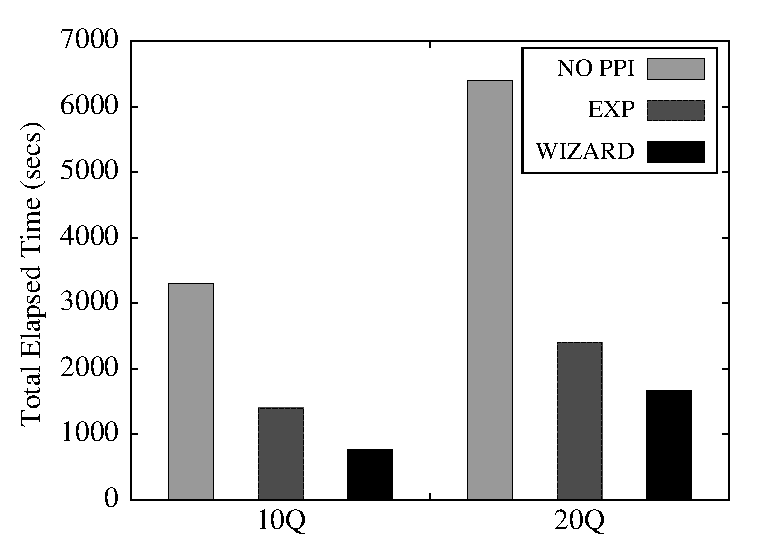
\includegraphics[scale=0.6]{3T_total_time}
	\label{fig:3T_eval_res}
}
\vspace{-0.1in}
\caption{Total Elapsed Time\label{fig:total_elapsed_time}}
\end{figure*}

\begin{figure*}[t]
\vspace{-.2in}
\centering
\subfigure[1TB]{
	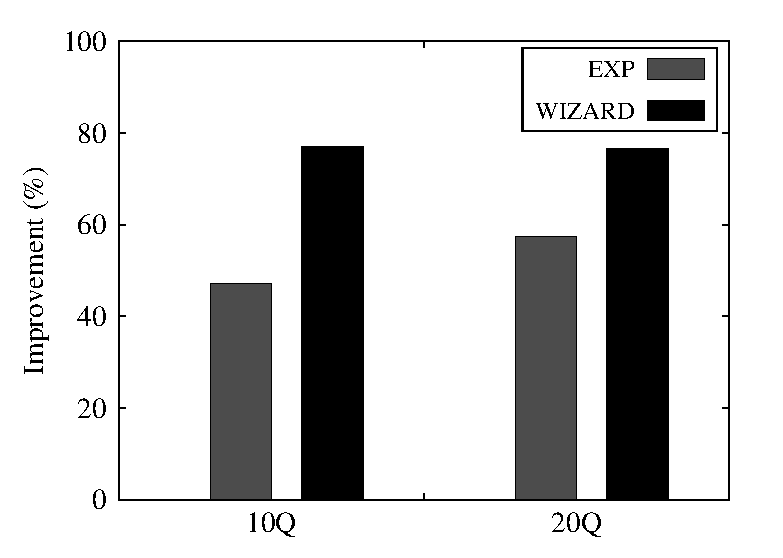
\includegraphics[scale=0.6]{1T_quality}
	\label{fig:1T_quality}
}
\subfigure[3TB]{
	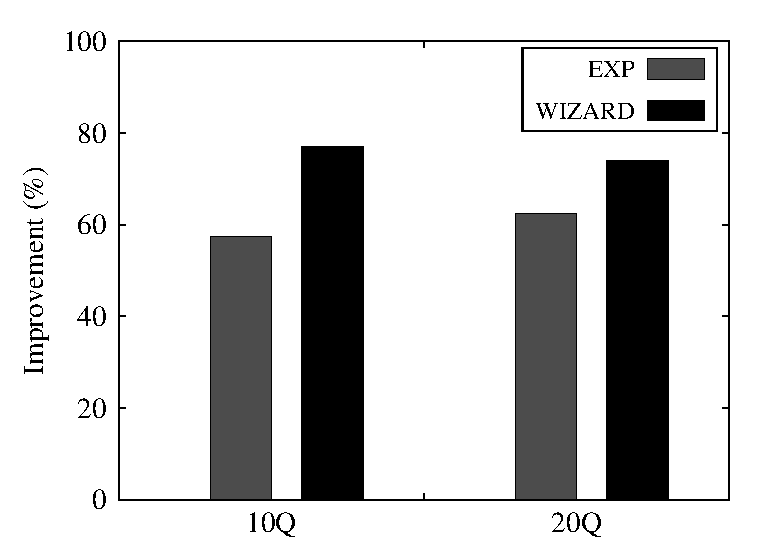
\includegraphics[scale=0.6]{3T_quality}
	\label{fig:3T_quality}
}
\vspace{-0.1in}
\caption{Recommendation Quality Comparison\label{fig:recomm_qual}}
\vspace{-.1in}
\end{figure*}

\subsection{Performance Evaluation}

The main focus of our demonstration is to see the performance (quality) 
of MLPPI recommendations made by the MLPPI wizard (WIZARD), 
compared with the performance of no partitioning (NO PPI) and EXP (partitioning 
by a human expert). 

%Our evalution results are exhibited in Figures ~\ref{fig:eval_res} 
%and ~\ref{fig:improvement}.
%Figure~\ref{fig:eval_res} shows the times (in seconds) taken 
%to run the 10Q or 20Q workloads over the 1TB or 3TB fact tables. 
%Based on the run results, Figure~\ref{fig:improvement} displays 
%how much improvement could be achieved by the EXP or the WIZARD 
%recommendations against the NO PPI one. 

Figures~\ref{fig:total_elapsed_time} and \ref{fig:recomm_qual} exhibit our evaluation results.
Figure~\ref{fig:total_elapsed_time} shows the times (in seconds) taken 
to run the 10Q and 20Q workloads over the 1TB and 3TB fact tables. 
Based on the run results, Figure~\ref{fig:recomm_qual} shows 
how much improvement was gained by the EXP and WIZARD solutions, compared with the NO PPI solution. 

Overall, the WIZARD recommendations were very effective at partitioning 
the fact tables by leveraging the predicates in the workloads. 
On average, the \hbox{total} execution time of the workloads on the WIZARD solutions was 
about 3.5 and 2 times faster than those of NO PPI and EXP, respectively. 
Also, the quality of the \hbox{WIZARD} solutions outperformed that of the EXP solutions; 
the WIZARD solutions yielded an average of about 77\% improvement on the NO PPI solutions.  

Furthermore, the WIZARD recommendations 
scaled very well with growing workload size and table size, 
as illustrated in Figure~\ref{fig:recomm_qual}. 
Although we doubled the workload scale from 10Q to 20Q, 
the performance improvement of the WIZARD solution stayed the same in Figure~\ref{fig:1T_quality} 
and got almost negligibly decreased in Figure~\ref{fig:3T_quality}. 
This result showed that our WIZARD \hbox{solution} was scalable over increasing workload size.

We also increased the table scale from 1TB to 3TB. 
For 10Q the performance improvement (about 77\%) was almost the same over the increasing scales, 
and for 20Q it was decreased from 76\% to 74\%, which was \hbox{almost} negligible.
The WIZARD partitioning \hbox{recommendation} scaled well with increasing table size.

In sum, our experiment results attest the effectiveness of the proposed algorithms for WIZARD 
and show the superiority of the recommendations of WIZARD.

\shorten{Regarding the scale of 1TB in Figure~\ref{fig:1T_quality}, 
although we doubled the workload scale (from 10Q to 20Q) 
the performance improvement of the WIZARD solution compared with that of NO PPI was not decrease although we doubled the workload scale (from 10Q to 20Q).
In Figure~\ref{fig:3T_quality}, for the 3TB scale the improvement of WIZARD was slightly decreased, but it was negligible.
In sum, the performance of the WIZARD solution was scalable over increasing workload and table scale. 

%Also, we scaled up the table from 1TB to 3TB on the fixed workload, but 
%the \hbox{recommendation} quality was not degraded at all. 
These results attest the effectiveness of our algorithms, 
and show the superiority of our recommendations.}

\section{Related Work}
\label{sec:related_work}

Physical database design~\cite{finkelstein1988physical,labio1997physical,rozen1991framework,Zilio1998} 
has been discussed in \hbox{academic} research and industrial sectors in the past years.
The major DBMS vendors (e.g., IBM, MS, and Oracle) have driven much of the work. 
Their specific interests have been in automating the physical design for table 
partitioning~\cite{agrawal04:integrating,Lightstone04:db2auto,nehme2011automated,sheet2009oracle,saa2007oracle,rao2002automating}, indexes/materialized views~\cite{agrawal2000automated,Agrawal04:sqlserver,dash2011cophy,Kimura11,itwsqlserver,valentin2000db2,zilio2004recommending}, 
and integration~\cite{Zilio04:db2design}.

%Lightstone's work~\cite{Lightstone04:db2auto} introduces the MDC (Multidimensional 
%Clustering) Advisor that automates the selection of MDC 
%keys customized for a specific workload on DB2 Universal Databases to use MDC structure. 
%DB2 Advisor~\cite{Zilio04:db2design} is an integrated commercial 
%tool that captures a variety of aspects of physical database design 
%by automation in a comprehensive way. 
%Oracle Partitioning Advisor~\cite{sheet2009oracle} for recommending 
%table partitionings is  integrated into 
%the SQL Access Advisor~\cite{saa2007oracle}. 

%Since data clustering significantly influences on the performance of 
%multidimensional queries, the MDC advisor helps DBAs that may have 
%nontrivial troubles in finding proper clustering dimensions and 
%granularity. 
%To enumerate and determine possible clustering dimensions, 
%his work relies on {\it what-if} query cost modeling, data sampling and a search algorithm. 

%DB2 Advisor~\cite{Zilio04:db2design} is an integrated commercial 
%tool that captures a variety of aspects of physical database design 
%by automation in a comprehensive way. 
%It makes an attempt to cover a variety of design choices-partitioning, 
%MDC, materialized views and indexes. 
%DB2 Advisor leverages the DB2 query optimizer for yielding a recommendation, and 
%takes a hybrid searching approach for considering different features.

%Oracle has a tool, called Partitioning Advisor~\cite{sheet2009oracle}, 
%to make a partitioning recommendation for tables. 
%The tool is now integrated into 
%the SQL Access Advisor~\cite{saa2007oracle} that recommends indexes and materialized 
%views. 
%However, its technical details are not yet released in public. 
%
%Also, MS SQL Server provides some similar, automated tools~\cite{agrawal2000automated,agrawal04:integrating,
%itwsqlserver} for table partitioning, materialized views or indexes fitting to a given workload.
%The optimizer cost model is exploited to acquire estimates for 
%candidate materialized views or indexes. 
%In particular, Agrawal's work~\cite{agrawal04:integrating} presents 
%an approach of integrating vertical and horizontal partitioning schemes 
%into their physical database design, considering scalability.

Some of the tools in IBM DB2~\cite{Lightstone04:db2auto}, 
Oracle~\cite{sheet2009oracle}, and MS SQL Server~\cite{agrawal04:integrating} 
appear to be similar to our MLPPI wizard. 
However, in light of problem scope and approach, the wizard 
is fundamentally different from the existing tools excluding Oracle Partitioning \hbox{Advisor}~\cite{sheet2009oracle} 
providing no published technical details. 

DB2 MDC Advisor~\cite{Lightstone04:db2auto} actually tackles 
a different problem of automatically recommending the most well-suited MDC 
keys for a given workload. 
Agrawal's work~\cite{agrawal04:integrating} 
discusses another problem of merging \hbox{single-level} range partitionings on objects such as tables and indexes. 
This article addresses the multi-level \hbox{partitioning} problem. 
Hence, the existing solutions cannot be directly applied to our MLPPI wizard.   

Regarding the approach, DB2 MDC Advisor~\cite{Lightstone04:db2auto} uses 
the search space driven by {\em fields}. In contrast, our search 
space is driven by query-predicates, which is superior because 
predicates are more customized and specific to a workload than fields. 

Agrawal's horizontal partitioning scheme~\cite{agrawal04:integrating} 
also uses the search space driven by simple range predicates, but 
his technique has a shortcoming as follows. 
His work produces a solution for each individual query and attempt 
to merge the solutions. But this approach cannot reach 
an optimized solution in a global perspective.
Our wizard generates the whole search space upfront and in turn merges partitions, leading to a \hbox{globally-optimized} solution. 
While his work considers a single column only, we deal with multiple fields.

Implementations of previous tools~\cite{agrawal04:integrating,Lightstone04:db2auto,nehme2011automated} \hbox{required} instrumentation for optimizer code.
These instrumentations are needed to facilitate the required 
information for the physical design tools API calls. 
The \hbox{instrumentation} code need to be enhanced and tested for new database 
releases that add complexity and additional cost for software upgrades. 
But our algorithm is based existing APIs supported by an optimizer (like Teradata), 
which requires no code change in the optimizer.
%The Teradata optimizer with a rich set of existing APIs originally coded 
%for system and workload management tools. 
%The APIs are sufficient to avoid the costly optimizer code change. 

Also, Nehme's work~\cite{nehme2011automated}, deeply-integrated with 
optimizer, reveals a concern about the quality of the recommendations 
made by some tools, shallowly integrated with optimizer. 
But we observed in our experiments that the quality of 
the wizard's solutions was much superior to that of the base solutions. 
In addition, some might argue that in our loosely-coupled approach 
the cost to invoke the optimizer might be significant. 
But the measured call counts were much fewer than 
the theoretical bound, since most calls were made only when queries were affected by a merge.  
%If the remote communication cost is expensive, the tool can also be run, 
%{\em co-located} with the server. 

%The existing work requires their database engine to be extended 
%to support their features. 
%This strong coupling may impose a nontrivial burden on their servers whenever 
%a new feature of the existing tools is desired. 
%As illustrated in Figure~\ref{fig:arch}, our tool is completely outside 
%the DBMS server. Thus, we are free of the constraint. 
%A literature~\cite{nehme2011automated} claims that 
%such loosely-coupled approaches might suffer from the reduced performance of a tool 
%and the poor quality of the partitioning recommendations. 
%The powerful Teradata APIs, however, help the wizard receive from the server 
%everything needed for yielding a MLPPI recommendation. 
%Moreover, as demonstrated in Figure~\ref{fig:perf_eval}, the quality of the 
%partitioning solutions by the wizard was also much superior to that of the base solutions.
%Some might argue that the cost of invoking the optimizer could be significant as well. 
%Again, the actual calls are mainly made only when queries are affected by a merge. 
%As a result, they were much fewer than 
%the theoretical bound as shown in Table~\ref{tab:workload_stat}.  
%To further save the remote communication cost, the tool can also be run, 
%{\em co-located} with the server. 
%Therefore, we believe that the shallowly-integrated strategy perfectly matches 
%with the wizard. 

Lastly, there has been some previous work~\cite{nehme2011automated,rao2002automating,tatarowicz2012lookup} 
regarding table partitioning in multi-node \hbox{systems}, but 
our problem is discussed in the context of a single node system, as in the existing work~\cite{agrawal04:integrating}. 
Database cracking~\cite{idreoskm07}
%, self-reorganizing column values in accordance with query workload, 
assumes a single node environment, but 
it does not address our multi-level partitioning problem. 

\section{Summary}
\label{sec:conclusion}
%We verified the effectiveness of the tool by running it on a workload based

Given workloads, it is difficult for DBAs to select appropriate fields 
in partitioning the fact table due to large search space. 
DBAs cannot easily determine how granular partitions should be made 
for the workloads. 

To address this concern, we presented the MLPPI wizard to recommend a fact-table partitioning for a given star schema workload. 
Since \hbox{query-predicates} are exploited 
to capture necessary ranges for fields and define partitions, 
the MLPPI \hbox{recommendation} can be very optimized, customized to the workload.  

We proposed the wizard's algorithms consisting of the three phases. 
The wizard incrementally reduced its search space by merging 
the range pair with the least scan or query cost, and eventually reached an MLPPI recommendation. 
In addition, we analyzed the running complexity for the initial and optimized phases. 
Despite the theoretically high bound, in practice, the wizard made much fewer calls in the phases.

We measured the performance of the recommendation by the wizard using 
our workloads.  
We demonstrated that the produced MLPPI solutions by 
the wizard could reduce the total elapsed time by more than a factor of two, 
compared with those of no partitioning approach and partitioning 
done by a human expert. 

%\section*{Acknowledgments} 
%This work was carried out while the first author visited Teradata. 
%The first author is now at Korea Institute of Science and Technology Information (yksuh@kisti.re.kr).

{\footnotesize
\bibliographystyle{splncs03}
\bibliography{paper}
}

\end{document}
